\section{Case Study: Autonomous Ground Support Equipment}
\label{sec:Case_Study}

This section briefly describes an Autonomous Ground Support Equipment (AGSE) robot that we designed, built, and deployed for the 2014-2015 NASA Student Launch Competition \cite{NASA_SL}. Special emphasis is given to the value of a rapid system prototyping methodology in the design process and how it allowed the AGSE to overcome many of the challenges and problems encountered during the competition.

\subsection{Competition Requirements}

The NASA Student Launch Initiative \cite{NASA_SL} is a research-based competition partnered with NASA's Centennial Challenges in order to stimulate rapid, low-cost development of rocket propulsion and space exploration systems.  Both collegiate and non-academic teams participate in the 8-month competition cycle composed of design, fabrication, and testing of flight vehicles, payloads, and ground support equipment. 

The purpose of the 2014-2015 competition was to simulate a Mars Ascent Vehicle (MAV) and to perform a sample recovery from the Martian surface. The requirements for this simulation were twofold: (1) Design and deploy an AGSE robot that autonomously retrieves a sample off the ground and stores it in the payload bay of a rocket, and (2) launch the rocket to an altitude of 3000 ft. before safely recovering the sample. 

While the driving requirements of the competition were fixed, many of the minor rules regarding AGSE performance, behavior, and safety requirements evolved and were augmented throughout the course of the eight month design cycle. The volatile nature of these rules precipitated the need for rapidly adjustable design and fabrication processes. For this purpose, the mechanical design of the AGSE followed a modular, quick-to-build approach and ROSMOD was used for software development in order to quickly make on-the-fly adjustments to system behavior.

\subsection{Mechanical Design}

The AGSE is a 4-DOF robot utilizing a revolute base joint to rotate the robot body, two prismatic joints to move vertically and horizontally, and a final revolute joint providing an orientation wrist for the end effector to orient a gripper. A wireframe and workspace rendering of the AGSE can be seen in Figure \ref{fig:Render}.

\begin{figure}[h]
	\centering
	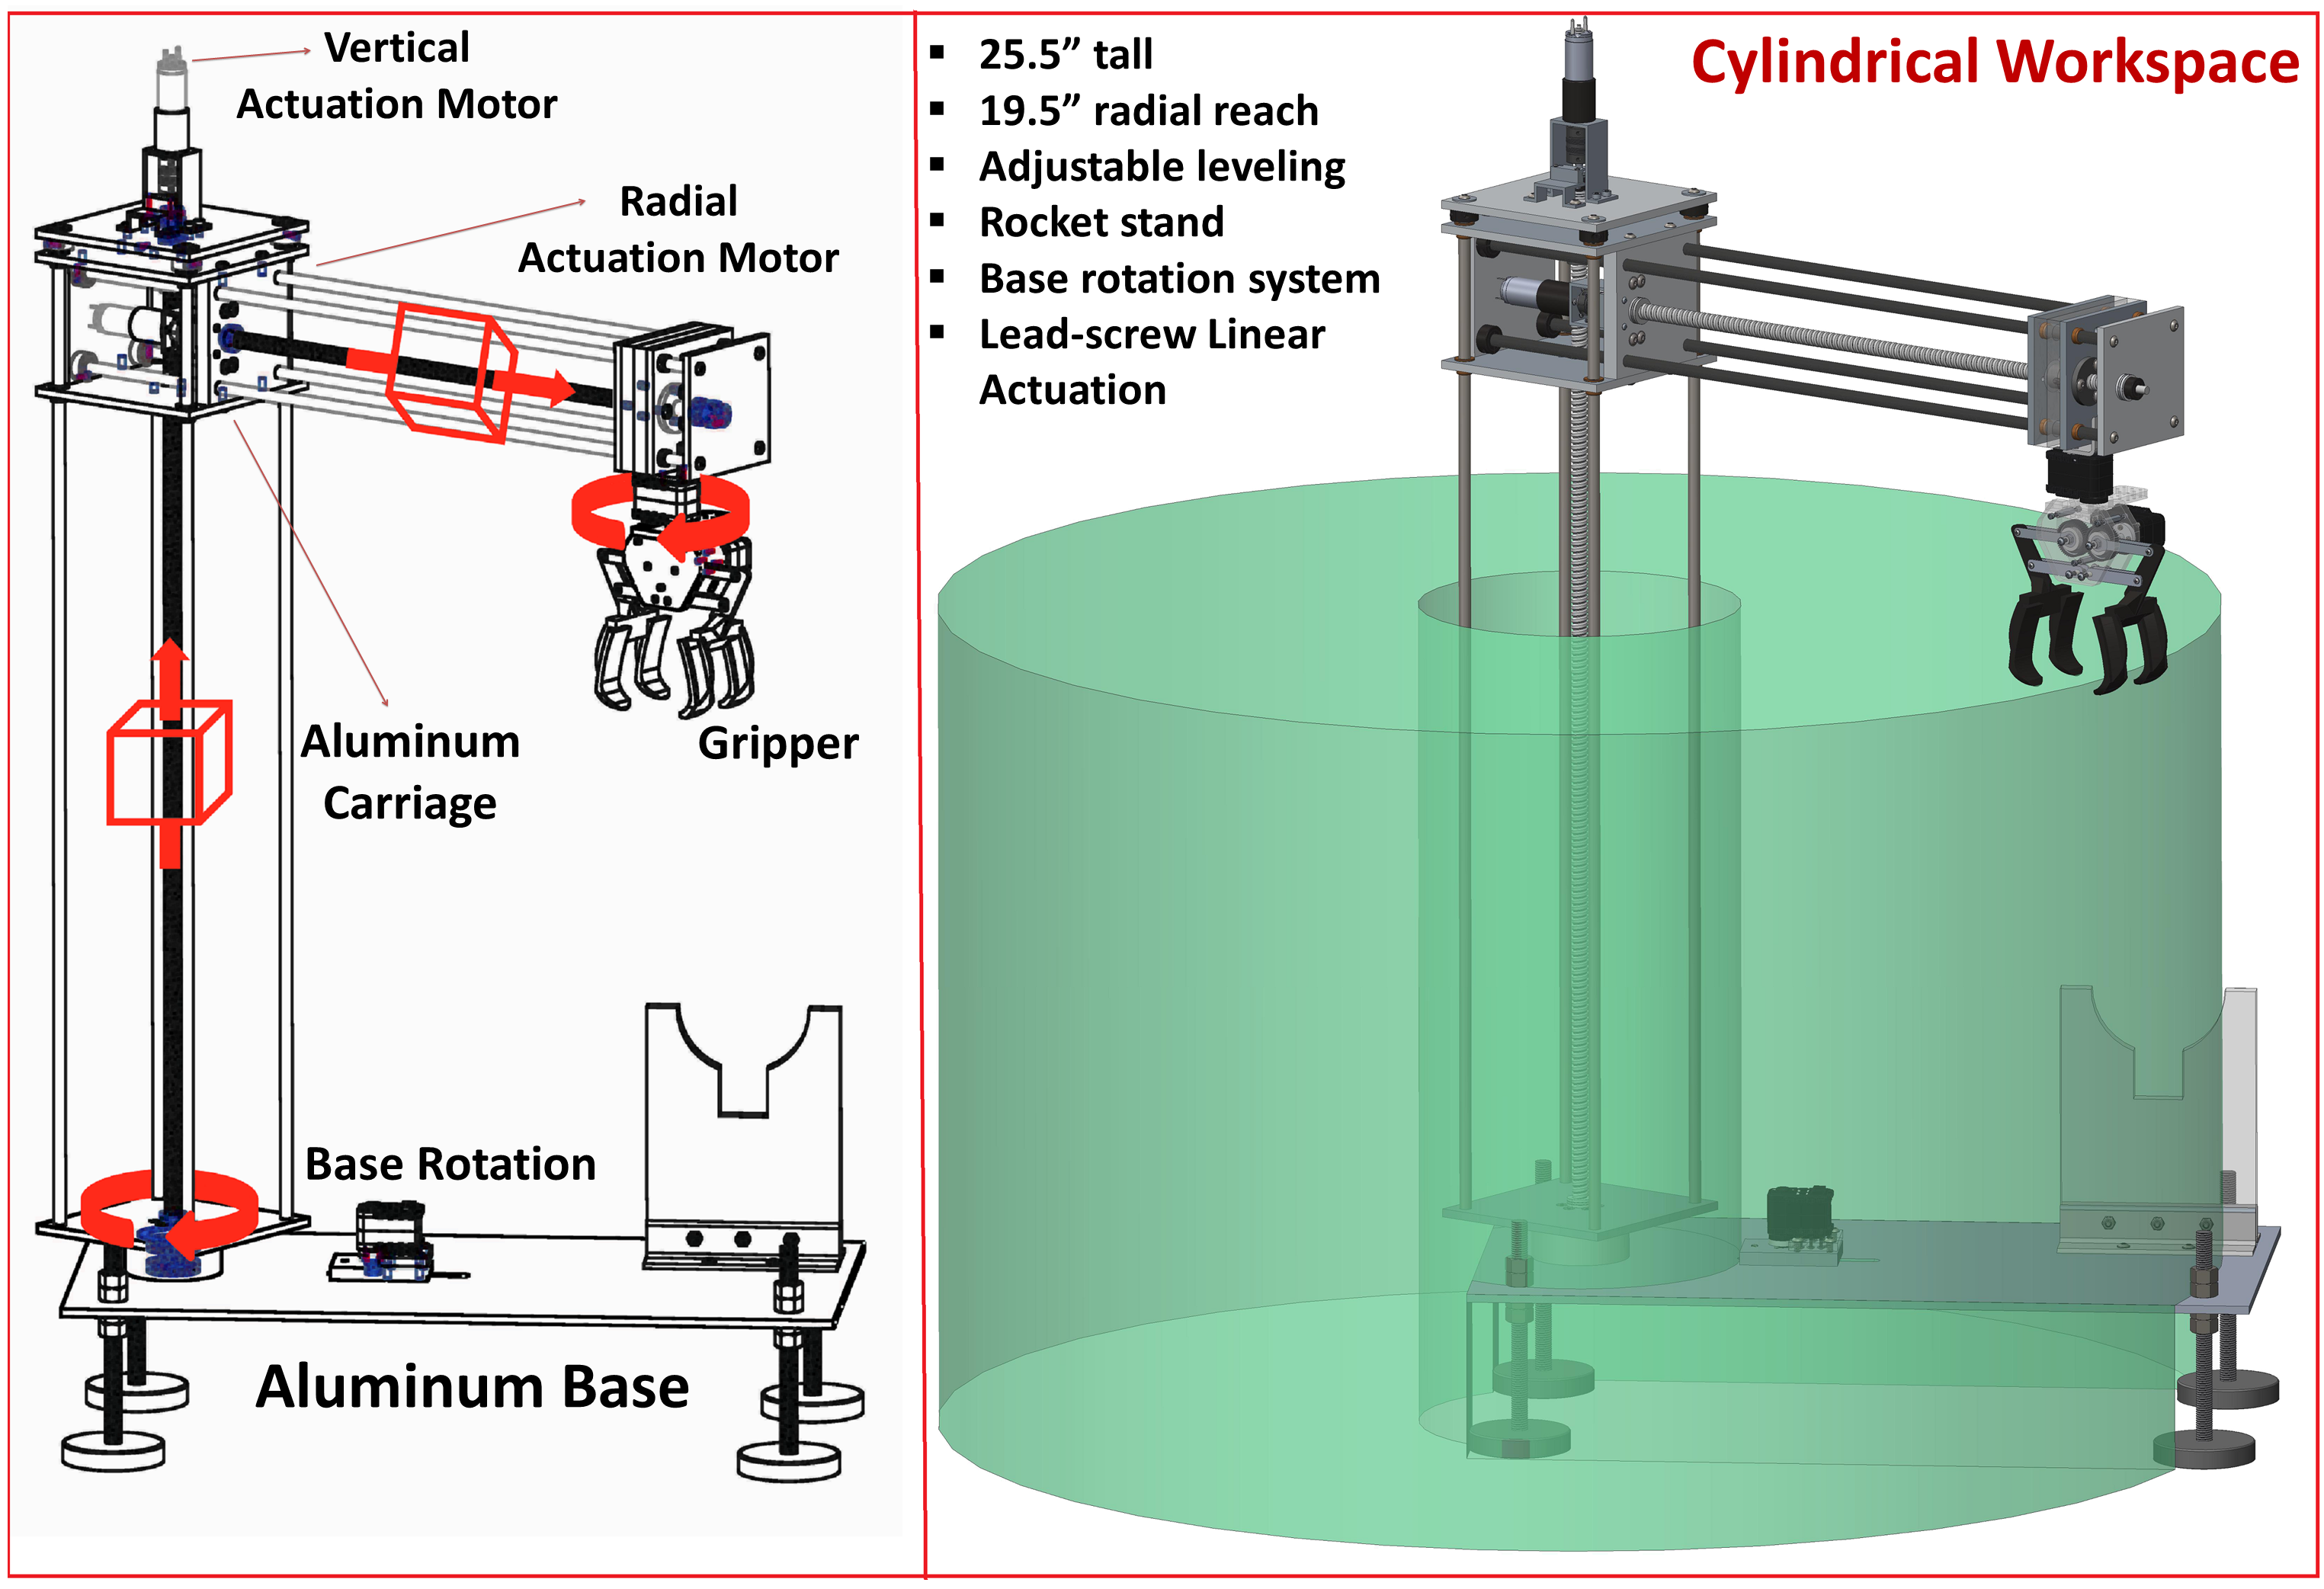
\includegraphics[width=0.48\textwidth]{figs/AGSE_Mechanical_Design_Figure.png}
	\caption{AGSE Mechanical Design}
	\label{fig:Render}
\end{figure}

The AGSE base is comprised of a machined sheet of aluminum, offering a secure mounting point for the upper robotic segments. Above this foundation level, a vertical lead screw, powered by a top-mounted DC motor, drives an aluminum carriage assembly up and down the central rotational axis. A similar lead screw-carriage assembly extends from the side of the vertical carriage to provide motion within the horizontal plane. The combined motion of these joints produces an open-cylindrical workspace. The radially actuating carriage connects to the end effector gripper via a wrist servo motor, which allows the AGSE to interact with the payload and rocket bay.

%The AGSE guides the end effector motion using the limit switch-encoder combo on its linear actuators, the built in positional feedback from the servo motors, and the optical feedback provided by a camera mounted above the end effector (allowing the AGSE to recognize objects within the reachable area underneath the gripper phalanges).

 %The AGSE base is comprised of a machined sheet of aluminum that offers a secure mounting point for the upper robotic segments, majority of the electronics, and the battery pack. Coincident with the base is the first revolute joint. This joint is operated by a servo motor directly coupled to the rotational axis. 
 
 %Vertical movement of the carriage is performed with respect to a limit switch (used to provide a zero reference position) located at the extreme upper limit of travel, and then tracked using an optical encoder to count revolutions of the lead screw.   

One significant set of challenges to the construction of the AGSE were time, machinist skill level, and the facilities available to the group's workforce. The team consisted mainly of undergraduate workers with limited machining experience and no access to CNC machinery.  Due to this constraint, the mechanical design and software needed to accommodate generous tolerance allowances in component machining. The system also needed to be robust enough to recover from the failure of a component, such as that detailed in Performance Assessment.

The short eight month duration of the design cycle, from initial planning to evaluation, meant that the AGSE system had to undergo rapid development.  As such, an iterative, modular, design-build-test approach was implemented in order to concurrently develop as many components of the hardware and software systems as possible. An initial AGSE prototype was conceptualized from off-the-shelf components and the mechanical and software systems were built in parallel, integrated, and tested. These preliminary results were then used in future development to produce a more ideal structure with greater positional accuracy and system robustness.  Due to the modular nature of the system's design, it was not necessary to immediately build a completely new second system, so incremental improvements could be made on a specific subsystem (such as the robot's gripper, any single degree of freedom, image processing, motor control, etc.) as the design evolved.
%\subsection{Image Processing}

%Periodic sample detection performed by the AGSE uses OpenCV-based image processing algorithms to identify and track the sample in real-time. An Image Processor component periodically fetches the latest feed from the mounted camera and performs a series of filtering tasks. 

%Each \emph{RGB} image frame is converted to both \emph{HSV} (hue-saturation-value) and \emph{Grayscale} image frames. After applying thresholds, filters, erosion and dilation methods, the target sample is extracted from the webcam feed. Once the target sample is detected, we draw contours around the object and identify its relative position and orientation. Figures \ref{fig:Sample_Image_Processing} and \ref{fig:Sample_Image_Processing_2} present our launch-day results. 

\subsection{Distributed Deployment}

The AGSE robot is controlled by a distributed set of embedded controllers. Figure \ref{fig:AGSE_Deployment} shows the high-level design for the deployment architecture. There are three embedded devices, each with its own responsibilities. 

\begin{figure*}[t]
	\centering	
	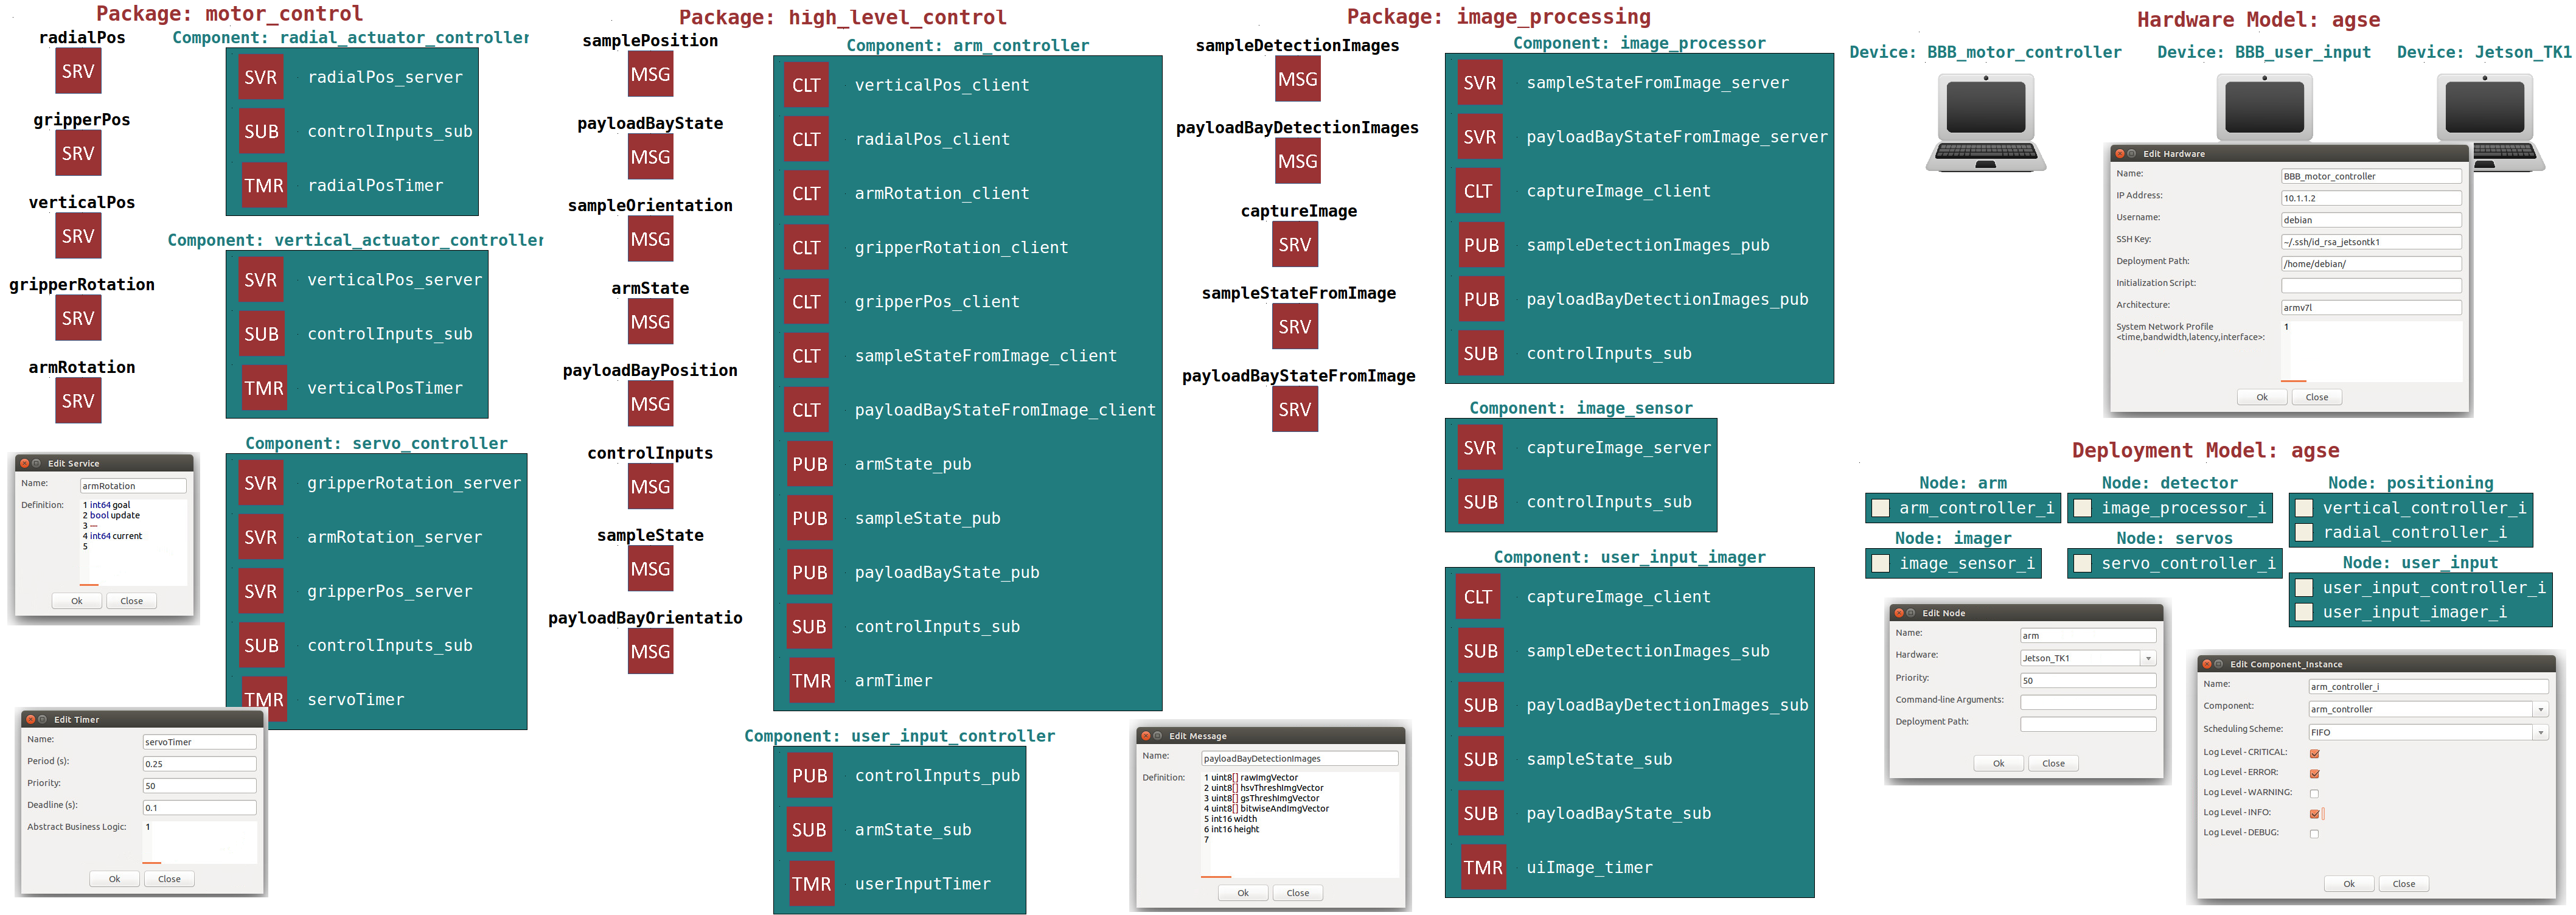
\includegraphics[width=1.0\linewidth]{figs/AGSE.png}
	\caption{AGSE ROSMOD Model}
	\label{fig:AGSE}	
\end{figure*}


An NVIDIA Jetson TK1 periodically fetches the latest webcam feed, performs image processing and high-level path planning, updating a global state machine. A Beaglebone black (BBB) mounted on top of the robot performs power management, low-level motor control and feedback processing. Lastly, a \emph{User Input Panel} houses a second Beaglebone Black, reacting to user input e.g. pause switch, touchscreen mode changes etc. This last controller is also responsible for keeping the user informed about the real-time state of the AGSE and the current webcam feed. Each of these controllers host ROS multiple nodes with ROSMOD component executor threads periodically performing algorithmic computations, calculating new robotic paths and maintaining the global state machine.

\begin{figure}[h]
	\centering
	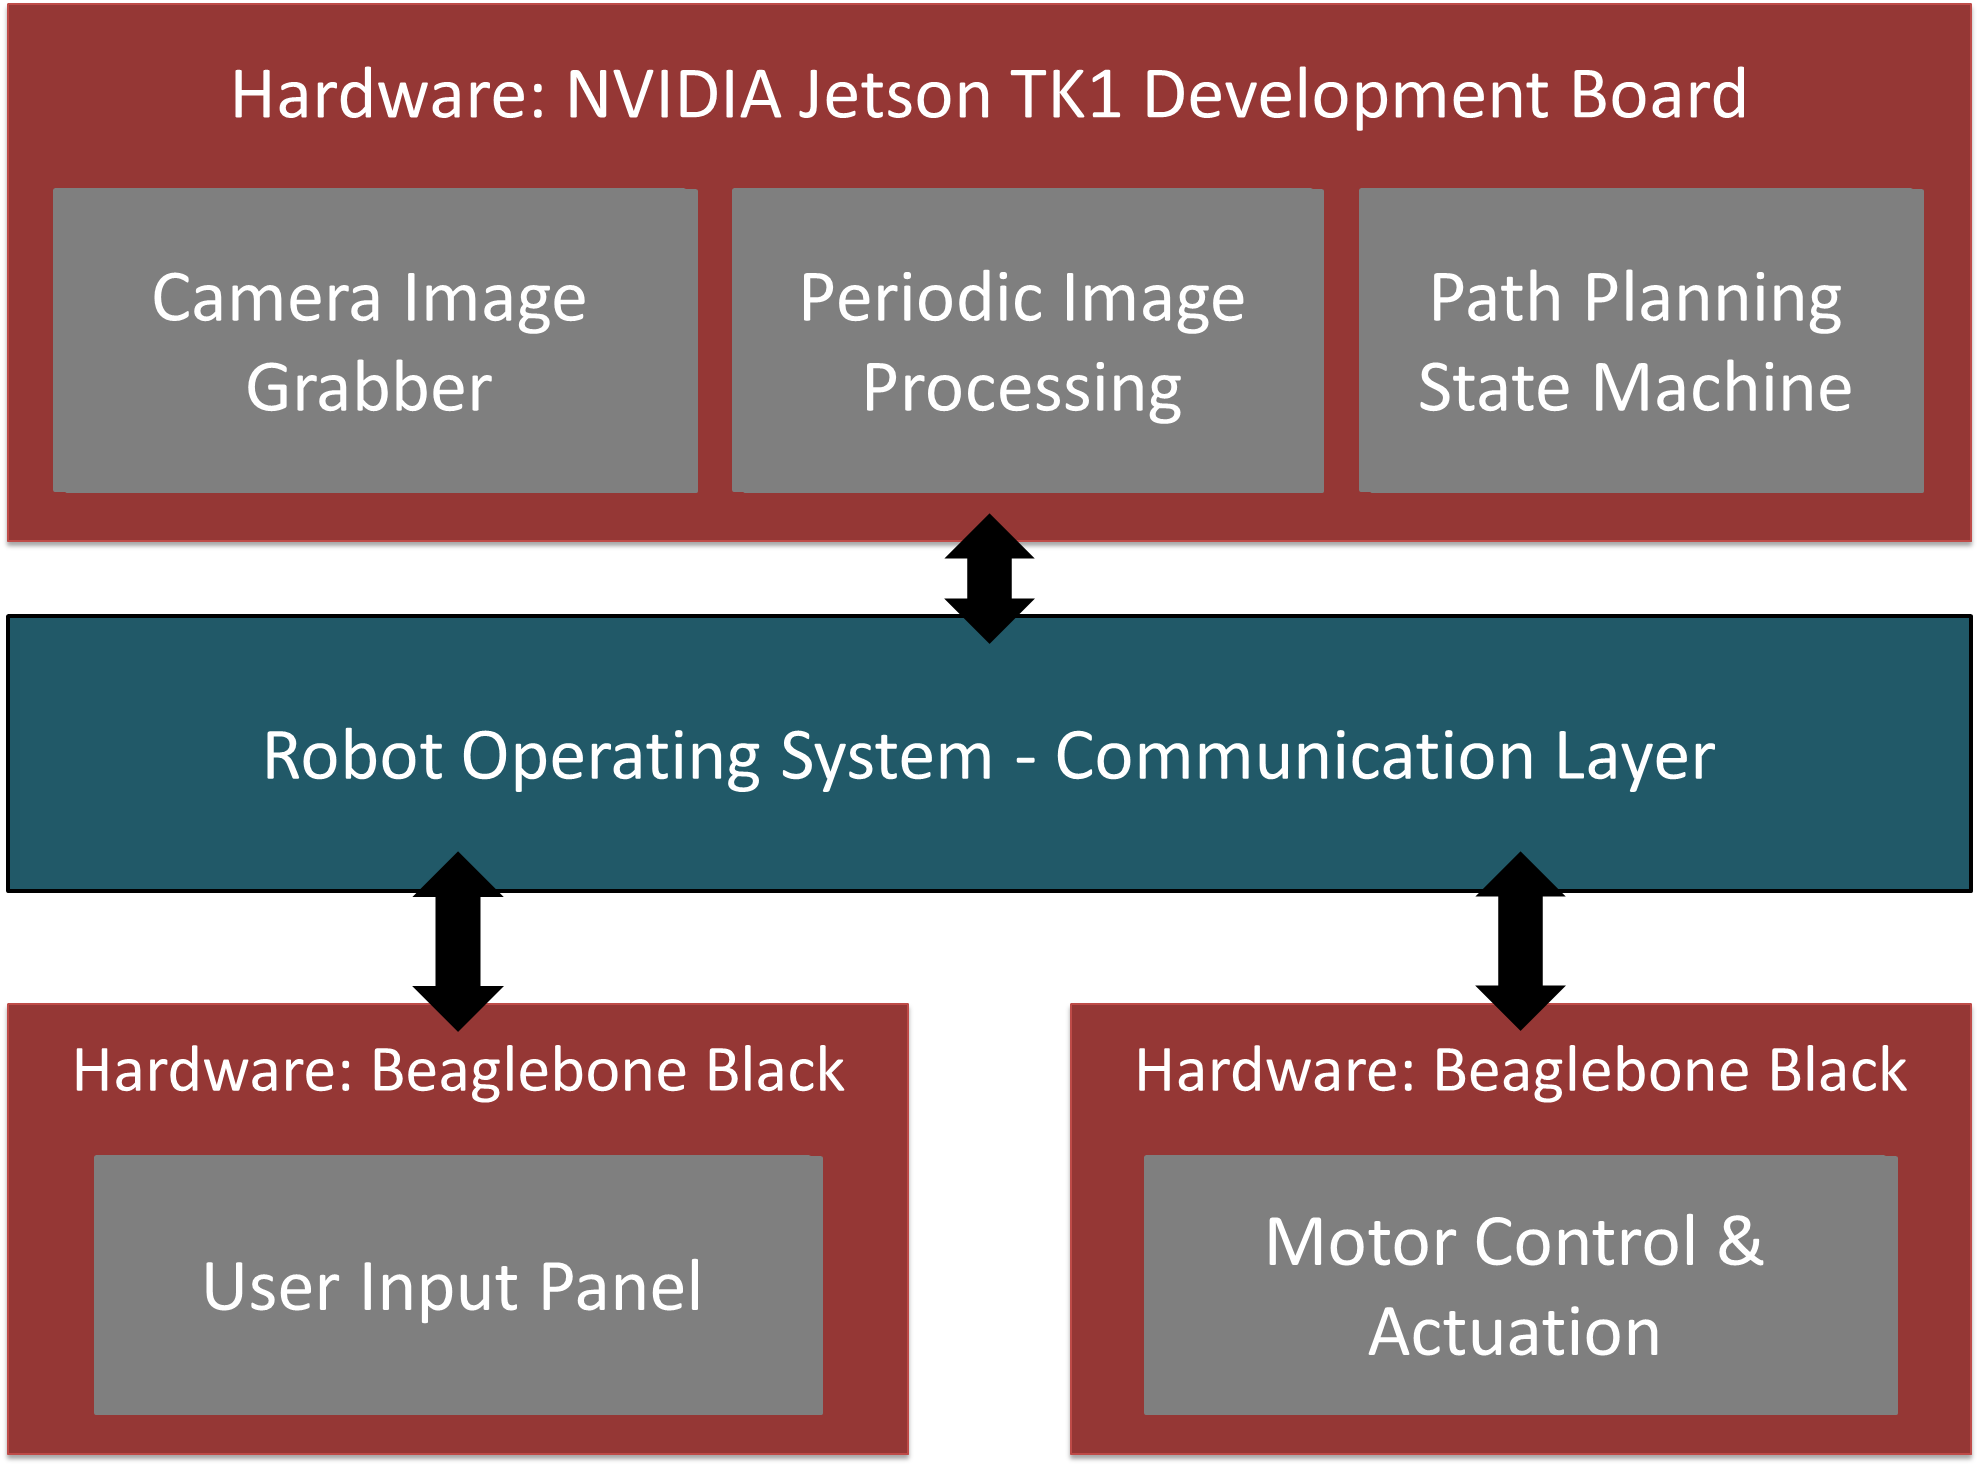
\includegraphics[width=0.45\textwidth]{figs/AGSE_Deployment.png}
	\caption{AGSE Package Deployment}
	\label{fig:AGSE_Deployment}
\end{figure}

\subsection{Software Prototyping with ROSMOD}

The AGSE software \cite{AGSE} was iteratively designed and rapid prototyped using ROSMOD. Figure \ref{fig:AGSE} shows the fully constructed ROSMOD models for the AGSE. The Software Model consists of 8 components spread across three ROS packages - motor control, high-level state machine control and image processing. Each package is characterized by its local set of messages, services and interacting components. 

The deployment model shows the various ROS nodes in the final system. Each node instantiates one or more components defined in the Software model e.g. the \emph{positioning} node executes two component threads, one behaving as a vertical\_actuator\_controller component and the other behaving as a radial\_actuator\_controller component. Each of these nodes is then deployed on one of the hardware devices modeled in the hardware model.

The ROSMOD code generators enabled generation of nearly 60\% (6,000+ lines) of the total built code. For systems like the AGSE with a medium-to-large set of interacting components, a small change to the message structure, port coupling, or functional dependencies can require a cascading and exponentially increased set of code changes. Typically, without ROSMOD, such code-breaking changes can cause a few days of work to fix and the build system can become brittle. This process can be cumbersome and error prone, especially when structural changes to software are frequent.

However, using ROSMOD's code generation and preservation features, such changes can be countered with a few seconds of code regeneration. As developers, we had to fill in the missing pieces - the business logic of the generated callbacks, completing the component interaction loops. This code includes architecture-specific control, e.g. GPIO and encoder readings, LED and switch settings, camera image acquisition, and high-level control. Although the overall software was frequently redesigned and tweaked, a large portion of this code required at most a few weeks of development and testing - a time frame that would not have been met without ROSMOD. 

\subsection{Performance Assessment}

At the competition, the Vanderbilt AGSE was able to complete the sample retrieval process in approximately $4.5$ minutes. The recovery process, as shown in Figure \ref{fig:AGSE_Operation}, was successful, with payload and rocket bay recognition occurring quickly and efficiently. The AGSE was able to grasp the payload using only two of its four padded end effector phalanges, and successfully deposited the payload within the rocket bay. This operation received high marks from the NASA officials and earned the competition's \emph{Autonomous Ground Support Equipment Award}.

System robustness was validated on the day of competition when a key component failed and was able to be quickly replaced with a different part with no detriment to system performance. The Dynamixel AX-12A servo controlling the base rotational degree of freedom of the AGSE suffered an irreparable failure of its gearbox and had to be removed from the robot. A backup of the servo was not readily available, and a different model servo by the same company had to be swapped in instead.  This new model, a Dynamixel MX-28T, while having similar performance as the old servo, had a different communication protocol and mounting footprint, as well as a more complex control scheme.

The component-based nature of ROSMOD allowed quick modifications of the business logic of the \emph{servo\_controller} package to update the system to use the new hardware.  The new control scheme was quickly implemented and the new physical placement of the servo due to its different mounting footprint was accounted for in software. After these modifications were made, the AGSE was able to perform at its optimal level during its part of the competition.

The rapid prototyping facilitated by ROSMOD and the ROS infrastructure enabled the development of an overall \emph{smarter} robot. The software requirements for autonomy were matched by the ROSMOD code generators such that developers had to spend little time setting up the build system and interaction patterns. The speed of development was drastically improved and the \emph{business logic} code, i.e. the core of the implementation of the system behavior, could be made more robust.


\begin{figure}[h]
	\centering	
	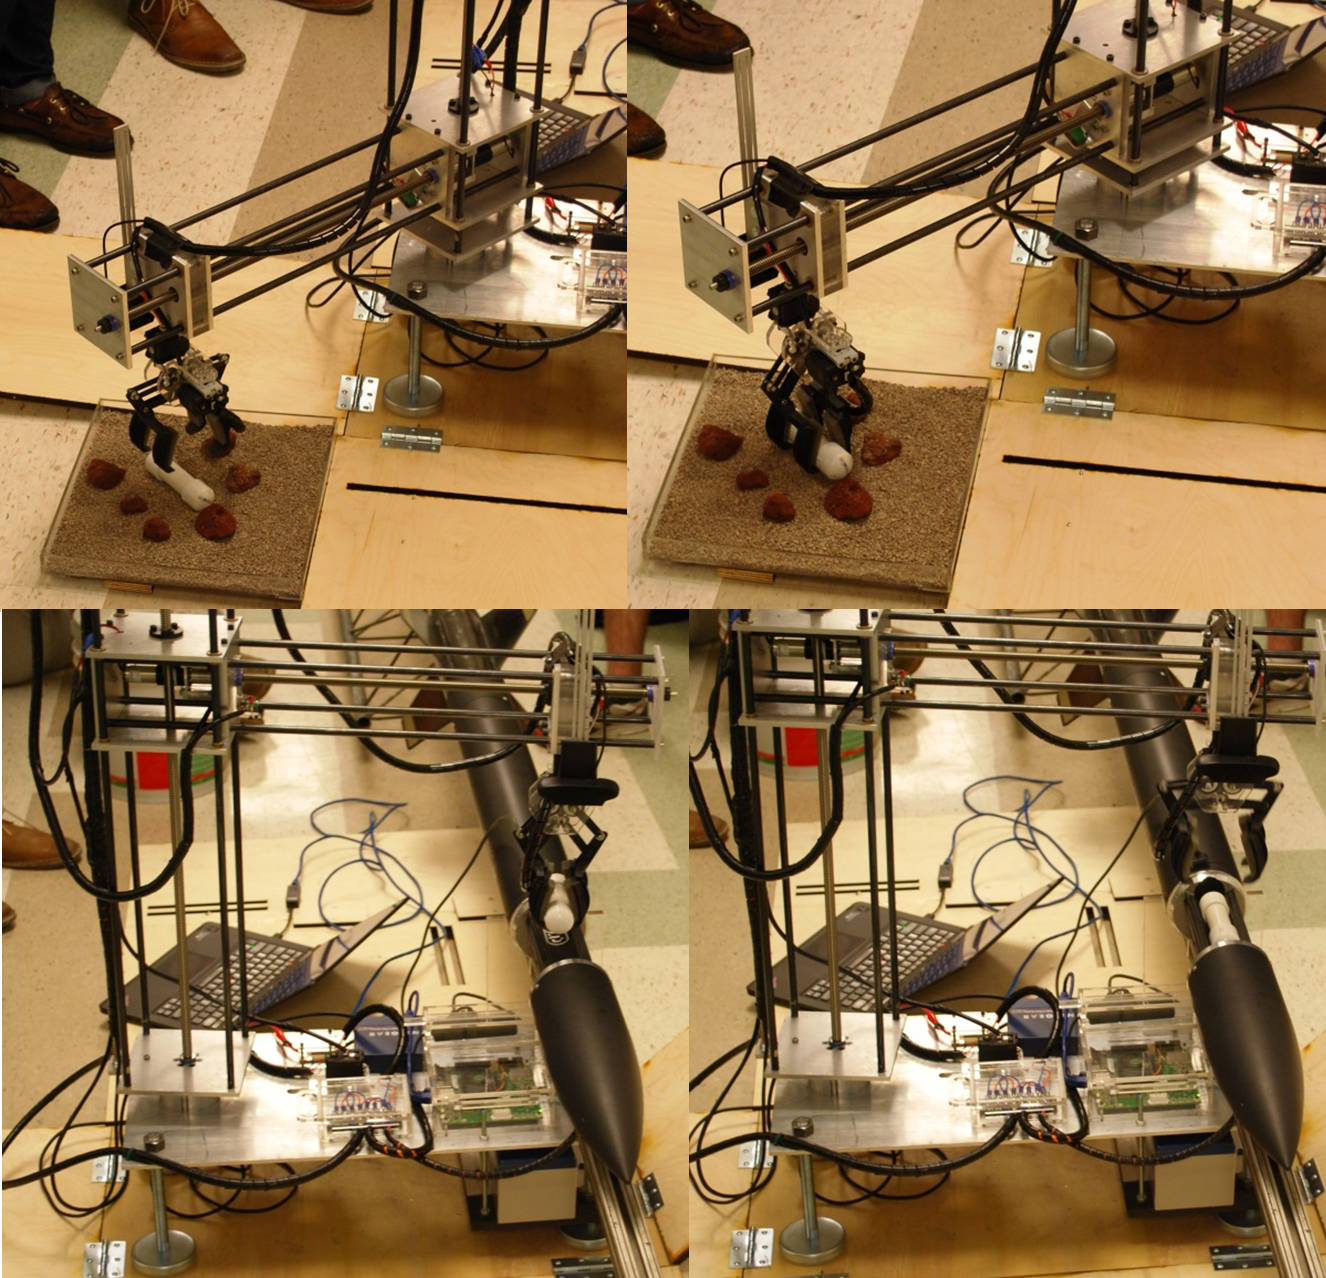
\includegraphics[width=1.0\linewidth]{figs/AGSE_Operation.png}
	\caption{AGSE Calibration and Testing}
	\label{fig:AGSE_Operation}	
\end{figure}
\vspace{-0.1in}

